\let\negmedspace\undefined
\let\negthickspace\undefined
\documentclass[journal,12pt,onecolumn]{IEEEtran}
\usepackage{cite}
\usepackage{amsmath,amssymb,amsfonts,amsthm}
\usepackage{algorithmic}
\usepackage{graphicx}
\graphicspath{{./figs/}}
\usepackage{textcomp}
\usepackage{xcolor}
\usepackage{txfonts}
\usepackage{listings}
\usepackage{enumitem}
\usepackage{mathtools}
\usepackage{gensymb}
\usepackage{comment}
\usepackage{caption}
\usepackage[breaklinks=true]{hyperref}
\usepackage{tkz-euclide} 
\usepackage{listings}
\usepackage{gvv}                                        
%\def\inputGnumericTable{}                                 
\usepackage[latin1]{inputenc}     
\usepackage{xparse}
\usepackage{color}                                            
\usepackage{array}
\usepackage{longtable}                                       
\usepackage{calc}                                             
\usepackage{multirow}
\usepackage{multicol}
\usepackage{hhline}                                           
\usepackage{ifthen}                                           
\usepackage{lscape}
\usepackage{tabularx}
\usepackage{array}
\usepackage{float}
\newtheorem{theorem}{Theorem}[section]
\newtheorem{problem}{Problem}
\newtheorem{proposition}{Proposition}[section]
\newtheorem{lemma}{Lemma}[section]
\newtheorem{corollary}[theorem]{Corollary}
\newtheorem{example}{Example}[section]
\newtheorem{definition}[problem]{Definition}
\newcommand{\BEQA}{\begin{eqnarray}}
\newcommand{\EEQA}{\end{eqnarray}}
\newcommand{\define}{\stackrel{\triangle}{=}}
\theoremstyle{remark}
\newtheorem{rem}{Remark}

\begin{document}

\title{12.277}
\author{ee25btech11056 - Suraj.N}
\maketitle
\renewcommand{\thefigure}{\theenumi}
\renewcommand{\thetable}{\theenumi}

\begin{document}

\textbf{Question :} Two points \((4,p)\) and \((0,q)\) lie on a straight line having a slope of \(3/4\). Find the value of \(p-q\).

\textbf{Solution :}

\begin{table}[h!]
  \centering
  \begin{tabular}{|c|c|}
\hline
\textbf{Name} & \textbf{Value} \\ \hline
$\vec{A}$ & $\myvec{2 & 1 \\0 & 3}$ \\ \hline
\end{tabular}

  \caption*{Table : Points}
  \label{12.277}
\end{table}

Let the equation of the line be  
\begin{align}
\vec{n}^\top \vec{x} = 1
\end{align}


$\vec{A}$ and $\vec{B}$ lie on the Line

\begin{align}
  \vec{n}^\top\vec{A} = 1\\
  \vec{n}^\top\vec{B} = 1
\end{align}


Stacking gives 

\begin{align}
\myvec{\vec{A} & \vec{B}}^\top \vec{n} = \myvec{1\\1}\\
\myvec{4 & p\\0 & q}\vec{n} = \myvec{1\\1}
\end{align}

Using back substitution we get $\vec{n}$ as 

\begin{align}
  \vec{n} = \myvec{\tfrac{q-p}{4q}\\\tfrac{1}{q}} = \myvec{\tfrac{q-p}{4}\\1}  
\end{align}

As the value of the slope of line is given in the question , we can write the normal vector as :

\begin{align}
  \vec{n} = \myvec{-\tfrac{3}{4}\\1} = \myvec{\tfrac{q-p}{4}\\1}   
\end{align}

From the above equation we get :

\begin{align}
p - q = 3
\end{align}

\textbf{Answer: } \(p-q = 3\)

\pagebreak

\begin{figure}[h!]
  \centering
  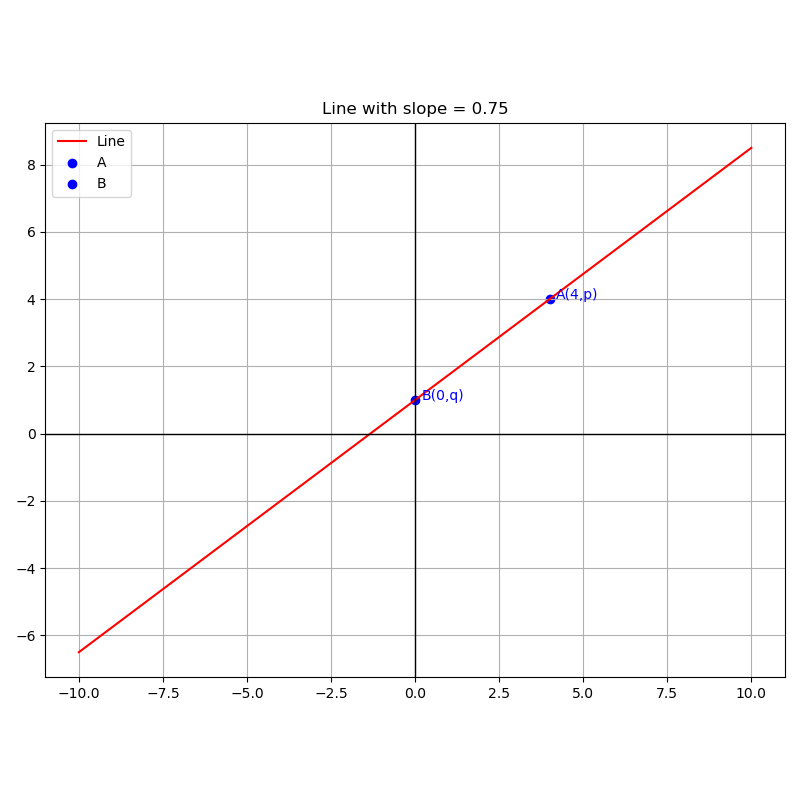
\includegraphics[width=0.7\columnwidth]{figs/line.png} 
   \caption*{Fig : Line}
  \label{Fig1}
\end{figure}

\end{document}

